\chapter{Architekturübersicht}
\section{Gesamtsystem und Komponenten}
Das entwickelte System basiert auf einer modularen client-server-Architektur, bei der verschiedene Komponenten logisch getrennt, aber technisch eng miteinander verknüpft agieren. Ziel ist es, eine wartbare, skalierbare und plattformunabhängige Anwendung bereitzustellen, die sich durch hohe Gebrauchstauglichkeit auszeichnet.
\begin{itemize}
    \item \textbf{Frontend (Client):} Das Frontend ist als Single Page Application (SPA) mit ReactJS umgesetzt. Es bietet die Benutzeroberfläche für Studierende und ermöglicht das Erstellen und Anzeigen von Vorlesungen, Notizen, Kalenderereignissen und To-Dos. Das Frontend greift über HTTP auf die REST-API des Backends zu.
    \item \textbf{Backend:} Das Backend ist in Node.js realisiert und stellt eine RESTful API bereit, die die Geschäftslogik der Anwendung kapselt. Es verarbeitet Anfragen vom Frontend, kommuniziert mit der Datenbank und führt die erforderlichen Operationen aus. Durch die Containerisierung in Docker ist eine konsistente Ausführung in verschiedenen Umgebungen gewährleistet.
    \item \textbf{Datenbank:} Die persistenten Daten werden in einer MySQL-Datenbank gespeichert. Diese läuft als Container innerhalb der Entwicklungs- und Produktionsumgebung. Die Datenbank enthält strukturierte Informationen zu Vorlesungen, Notizen, Kalenderereignissen und Stundenplaneinträgen. Das relationale Datenmodell erlaubt eine logische Trennung der Entitäten und eine effiziente Verarbeitung auch großer Datenmengen.
    \item \textbf{Dateispeicherung:} Hochgeladene Datein (z.B. PDF-Dokumente im Notizmodul) werden im lokalen Uploads-Verzeichnis des Servers gespeichert. Dieses Verzeichnis wird über einen statischen Pfad (/uploads) öffentlich bereitgestellt.
\end{itemize}
\section{Technologiestack}
In diesem Abschnitt werden die verwendeten Technologien beschrieben.
\subsection{ReactJS}
React ist eine Open-Source-JavaScript-Bibliothek, die dem User ermöglicht, Benutzeroberflächen aus einzelnen, wiederverwendbaren Komponenten zu erstellen. Mit React lassen sich sowohl klassische Web-UIs als auch native Benutzeroberflächen für Mobil- und Desktop-Apps realisieren, indem die gleichen Konzepte und das gleiche API-Design genutzt werden, so bleibt der Workflow plattformübergreifend konsistent und effizient. \autocite{react}
\subsection{PWA}
Eine Progressive Web App (PWA) ist eine Webanwendung, die moderne Webtechnologien wie HTML, CSS und JavaScript nutzt, um das Nutzungserlebnis einer nativen mobilen App nachzuahmen. Dabei kann sie über einen gewöhnlichen Webbrowser aufgerufen werden, lässt sich jedoch auch wie eine klassische App auf dem Startbildschirm eines Geräts installieren. PWAs zeichnen sich durch Eigenschaften wie Offline-Funktionalität, schnelle Ladezeiten, Push-Benachrichti-gungen und eine für mobile Endgeräte optimierte Benutzeroberfläche aus. Ziel ist es, die Vorteile von Websites mit denen nativer Apps zu kombinieren und somit eine plattformübergreifende, gebrauchstaugliche Lösung bereitzustellen. \autocite{pwa}
\subsection{Node.js}
Node.js ist eine offene, plattformübergreifende JavaScript-Laufzeitumgebung, die es ermöglicht, JavaScript nicht nur im Browser, sondern auch auf Servern, in Kommandozeilen-Tools und Skripten einzusetzen. Node.js bietet Entwicklern eine moderne, ereignisorientierte Plattform zur Erstellung hochskalierbarer Netzwerkapplikationen, ohne komplexe Thread-Verwaltung oder Blocking-I/O-Pro-bleme. \autocite{nodejs}
\subsection{MySQL}
MySQL ist ein weit verbreitetes, quelloffenes relationales Datenbankmanagementsystem (RDBMS). Es speichert strukturierte Daten in Tabellen mit expliziten Zeilen und Spalten, die durch Schemata definiert sind. Abfragen und Manipulation erfolgen über die standardisierte Sprache SQL (Structured Query Language). MySQL unterstützt ACID-konforme Transaktionen, was für sichere und zuverlässige Datenverarbeitung sorgt. Dank seiner hohen Leistung, Skalierbarkeit und der großen Entwickler-Community eignet sich MySQL sowohl für kleine Anwendungen als auch für internationale Webseiten, Webdienste und Unternehmenssysteme. \autocite{mysql}
\subsection{Docker}
Docker ist eine Plattform für Betriebssystemvirtualisierung, die Anwendungen in sogenannten Containern verpackt. Diese Container enthalten nicht nur die Anwendung selbst, sondern auch alle benötigten Abhängigkeiten. Im Gegensatz zu VMs teilen sich Container den Kernel des Host-Systems, was sie deutlich leichter und schneller macht. Images dienen dabei als Bauvorlagen und Container laufen als deren Instanzen. Docker unterstützt eine konsistente Portabilität über verschiedene Umgebungen hinweg und ermöglicht skalierbare, isolierte Anwendungsbereitstellung. Registry-Services wie Docker Hub erlauben das Teilen und Verwalten von Images. Zusätzlich bieten Tools wie Docker Compose die Orchestrierung mehrerer Container innerhalb komplexerer Anwendungen. \autocite{docker}
\section{Datenmodell und Datenbank}
Zur strukturierten und konsistenten Verwaltung der Anwendungsdaten wird ein relationales Datenmodell verwendet. Die Datenbank bildet das Rückgrat für die Speicherung von Informationen zu Vorlesungen, Notizen und Kalendereinträgen.\\
Zum Einsatz kommt eine MySQL-Datenbank, da dieses System weit verbreitet, gut dokumentiert und durch seine stabile Performance besonders geeignet für webbasierte Anwendungen ist. Die Datenbank läuft als eigenständiger Docker-Container und ist über eine REST-API mit dem Backend verbunden.\\
Für die Verwaltung und Speicherung der Anwendungsdaten wird eine relationale Datenbankstruktur verwendet, die mit MySQL umgesetzt wurde. Das Datenmodell ist in mehrere logisch getrennte Entitäten gegliedert und orientiert sich an den funktionalen Anforderungen der Webanwendung. Die folgende Grafik zeigt den schematischen Aufbau des Datenbanksystems:
\begin{figure}[H]
  \centering
  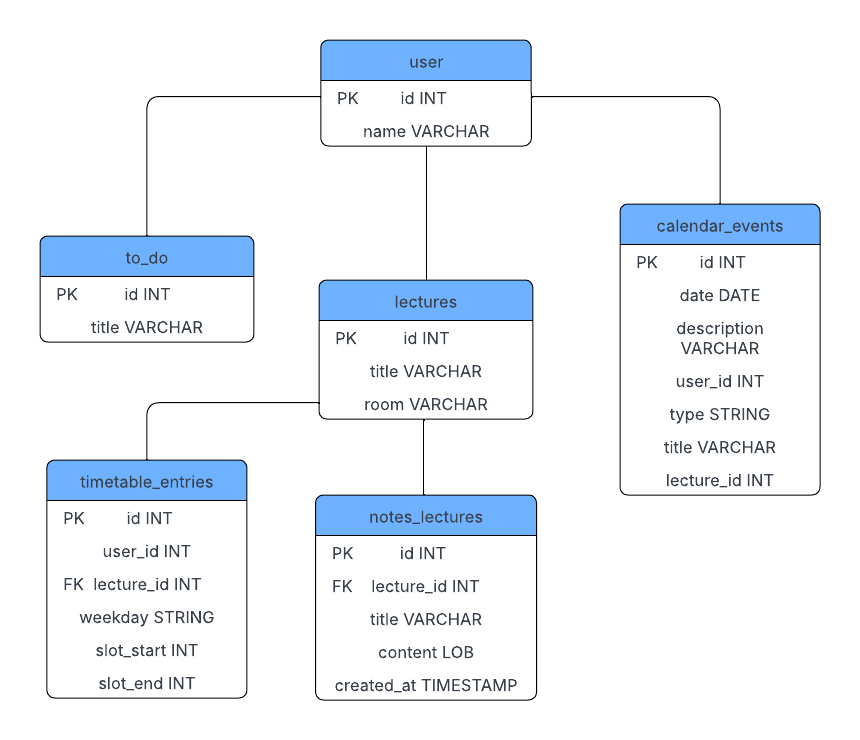
\includegraphics[width=1\textwidth]{./images/datenbankmodell.png}
  \caption{Datenbankmodell}
  \label{fig:datenbankmodell}
\end{figure}

\textbf{Entitäten und Beziehungen:}
\begin{itemize}
    \item \textbf{user:} Enthält Informationen zu den registrierten Nutzer:innen. Nutzer:innen können mehrere Vorlesungen, Notizen, Kalenderereignisse und To-Do-Einträ-ge besitzen.
    
    \item \textbf{lectures:} Repräsentiert einzelne Vorlesungen. Jede Vorlesung kann mit mehreren Notizen und Stundenplaneinträgen verknüpft sein.
    
    \item \textbf{notes\underline{ }lectures:} Speichert zu einer bestimmten Vorlesung gehörende Notizen mit Titel, Inhalt und Zeitstempel. Die Beziehung zu \texttt{lectures} erfolgt über einen Foreign Key.
    
    \item \textbf{calendar\underline{ }events:} Enthält Ereignisse wie Prüfungen, Abgaben oder Termine.
    
    \item \textbf{timetable\underline{ }entries:} Bildet konkrete Stundenplaneinträge ab. Neben der Vorle-sungs-ID werden auch Wochentag, Start- und Endzeit gespeichert.
    
    \item \textbf{to\underline{ }do:} Dient der Verwaltung einfacher Aufgabenlisten, die einem Nutzer:in-nen zugeordnet sind.
\end{itemize}
\textbf{Vorteile der Struktur:}
\begin{itemize}
    \item \textbf{Erweiterbarkeit:} Neue Funktionalitäten (z.B. Gruppen oder Tags) lassen sich durch zusätzliche Entitäten ohne größere Änderungen realisieren.
    \item \textbf{Skalierbarkeit:} Die klaren Beziehungen ermöglichen effiziente Abfragen, auch bei großen Datenmengen.
    \item \textbf{Wartbarkeit:} Die logische Trennung der Daten erhöht die Übersichtlichkeit und erleichtert Änderungen am Datenmodell.
\end{itemize}

\section{API-Design}
Die Kommunikation zwischen Frontend und Backend erfolgt über eine RESTful API, die auf dem HTTP-Protokoll basiert. Die Daten werden im JSON-Format übertragen. Die API stellt Endpunkte für die zentralen Funktionen der Anwendung bereit, wie das Erstellen und Abrufen von Vorlesungen, Notizen, Kalenderereignissen und Aufgaben.\\
\begin{longtable}{|p{6cm}|p{2cm}|p{6cm}|}
\hline
\textbf{Endpoint} & \textbf{Methode} & \textbf{Beschreibung} \\
\hline
/api/events & GET & Lädt alle Kalendereinträge, optional gefiltert nach \texttt{user\_id} und \texttt{type}. \\
\hline
/api/events & POST & Erstellt einen neuen Kalendereintrag mit Datum, Titel, Beschreibung usw. \\
\hline
/api/events/:id & DELETE & Löscht einen Kalendereintrag anhand seiner ID. \\
\hline
/api/lectures & GET & Gibt eine Liste aller Vorlesungen zurück. \\
\hline
/api/lectures & POST & Fügt eine neue Vorlesung mit Titel und Raum hinzu. \\
\hline
/api/lectures/:id & GET & Gibt eine bestimmte Vorlesung anhand ihrer ID zurück. \\
\hline
/api/lectures/:id & DELETE & Löscht eine Vorlesung anhand ihrer ID. \\
\hline
/api/timetable & POST & Fügt einen Stundenplaneintrag für einen bestimmten Nutzer hinzu. \\
\hline
/api/timetable/:user\_id & GET & Gibt den vollständigen Stundenplan eines Nutzers zurück. \\
\hline
/api/timetable/:id & DELETE & Löscht einen Stundenplaneintrag anhand seiner ID. \\
\hline
/api/to\_do & POST & Fügt einen neuen To-Do-Eintrag hinzu. \\
\hline
/api/to\_do & GET & Lädt alle To-Do-Einträge. \\
\hline
/api/to\_do/:id & DELETE & Löscht einen bestimmten To-Do-Eintrag. \\
\hline
/api/notes\_lectures & POST & Lädt eine neue Notiz zu einer Vorlesung hoch (PDF + Titel). \\
\hline
/api/notes\_lectures & GET & Lädt alle Notizen, sortiert nach Erstellungsdatum. \\
\hline
/api/notes\_lectures/:lecture\_id & GET & Lädt alle Notizen zu einer bestimmten Vorlesung. \\
\hline
/api/notes\_lectures/:id & DELETE & Löscht eine hochgeladene Notiz anhand ihrer ID. \\
\hline
\end{longtable}

Die grundsätzliche Systemarchitektur ist in Abbildung \ref{fig:systemarchitektur} dargestellt. Sie zeigt die Interatkion zwischen den drei Hauptkomponenten der Anwendung: dem ReactJS-basierten Frontend, dem containerisierten Node.js-Backend sowie der My-SQL-Datenbank. Die Kommunikation erfolgt dabei über standardisierte HTTP- und SQL-Schnittstellen. Auch der Prozess des Datei-Uploads ist visualisiert: Hochgeladene Dokumente werden vom Frontend an das Backend übermittelt und dort im Verzeichnis \texttt{/uploads} gespeichert, auf das wiederum das Frontend zur Anzeige zugreift.
\begin{figure}[H]
  \centering
  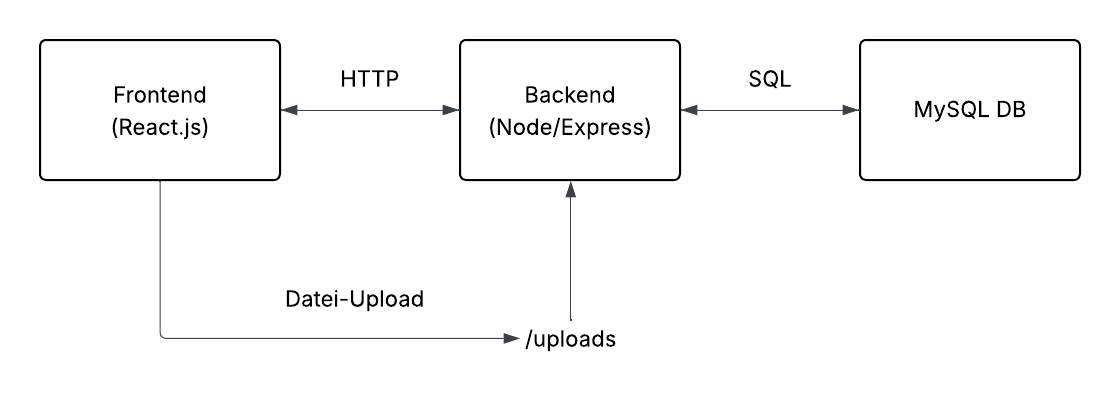
\includegraphics[width=1\textwidth]{./images/systemarchitektur.png}
  \caption{Systemarchitektur}
  \label{fig:systemarchitektur}
\end{figure}
